\section{Resultados}

% LES COPIO LO QUE TENIA EN EL CUADERNO:
% 	Delays en distintos momentos del dia? 
%	Se congestionan los enlaces en horas pico? (ver cuales son las horas pico en cada pais del enlace). 
%	Se utilizan los enlaces si voy a otras paginas cercanas a las que probamos? 
%	Cambian las rutas que se toman a una misma pagina? 
%	Ver tiempos de encolamiento (hacer algun tipo de analisis sobre esto supongo)

%Los datos de los siguientes graficos se midieron utilizando el Traceroute implementado por nosotros. El metodo de medicion fue el siguiente:
Utilizando el \texttt{traceroute} implementado por nosotros, y las herramientas de localizaci\'on mencionadas, observamos los siguientes enlaces transoce\'anicos:

\begin{itemize}
 \item Enlace 1: Entre Estados Unidos (Florida seg\'un \emph{IP2Location}, Colorado seg\'un \emph{IPLigence}), e Inglaterra (seg\'un \emph{IP2Location}), que detectamos rastreando la ruta hacia \url{www.helsinki.fi} (IP: 128.214.222.4, Finlandia).
 \item Enlace 2: Entre Estados Unidos, Colorado (seg\'un \emph{IPligence}) y Alemania (seg\'un \emph{IPligence}), detectado en el camino a \url{www.ox.ac.uk} (IP: 163.1.60.42, Reino Unido).
 \item Enlace 3: Entre Estados Unidos, Colorado (seg\'un \emph{IPligence}) y Zurich, Suiza (seg\'un todas las herramientas consultadas), detectado rastreando la ruta hacia \url{web.up.ac.za} (IP: 137.215.78.74, Sud\'africa).
\end{itemize}

Estos enlaces se corresponden con las siguientes IPs:

\begin{itemize}
 \item Enlace 1:\\
    IP en Am\'erica (EEUU): 67.17.106.162\\
    IP en Europa (Reino Unido): 213.155.137.26
  \item Enlace 2:\\
    IP en Am\'erica (EEUU): 67.16.139.18\\
    IP en Europa (Alemania): 141.136.107.37
  \item Enlace 3:\\
    IP en Am\'erica (EEUU): 146.82.32.154\\
    IP en Europa (Suiza): 77.109.134.50
\end{itemize}


En las figuras \ref{fig:mapa_fin}, \ref{fig:mapa_ing} y \ref{fig:mapa_sud} se muestra una localizacion aproximada de los enlaces transoceánicos utilizados.\\

\begin{figure}[H]
  \centering
    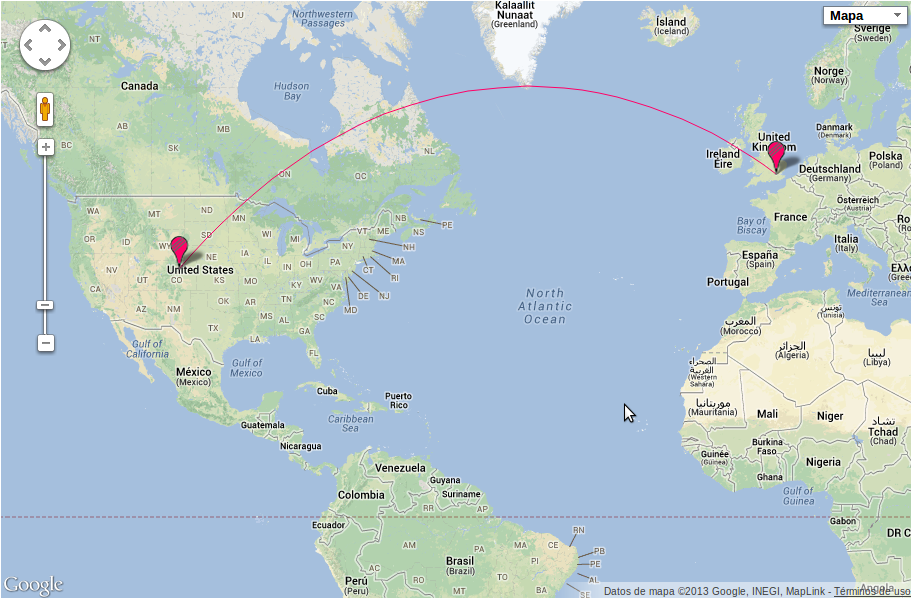
\includegraphics[width=0.9\textwidth]{imgs/finlandia_enlace_1.png}
    \caption{Mapa con la ubicacion aproximada del enlace tomado hacia el host \url{www.helsinki.fi} (Finlandia)}
    \label{fig:mapa_fin}
\end{figure}    

\begin{figure}[H]
  \centering
    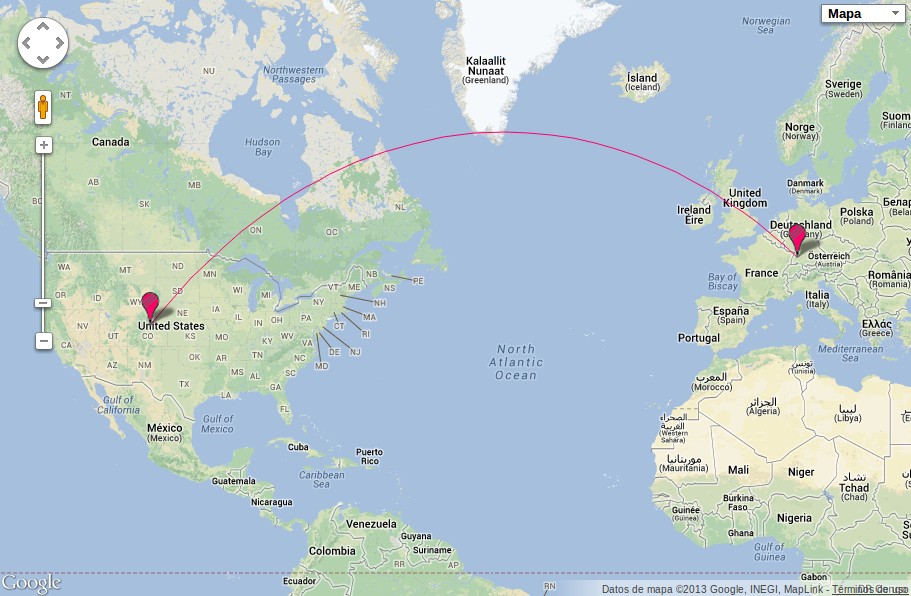
\includegraphics[width=0.9\textwidth]{imgs/inglaterra_enlace_1.png}
    \caption{Mapa con la ubicacion aproximada del enlace tomado hacia el host \url{www.ox.ac.uk} (Reino Unido)}
    \label{fig:mapa_ing}
\end{figure}

\begin{figure}[H]
  \centering
    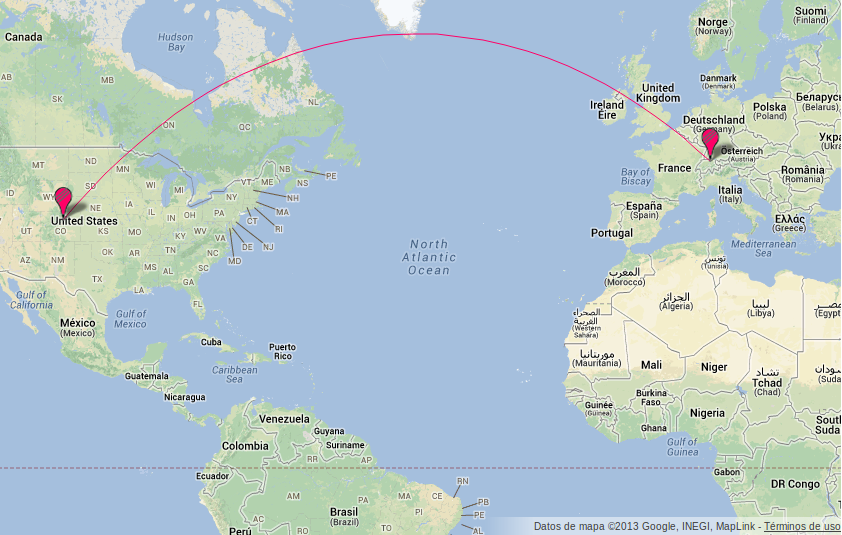
\includegraphics[width=0.9\textwidth]{imgs/sudafrica_enlace_1.png}
    \caption{Mapa con la ubicacion aproximada del enlace tomado hacia el host \url{web.up.ac.za} (Sud\'africa)}
    \label{fig:mapa_sud}
\end{figure}

Las figuras muestran claramente que los enlaces encontrados son aproximados, ya que recorren una distancia por tierra que no esta siendo considerada por el \texttt{traceroute}. Es muy probable que en el camino entre los enlaces encontrados existan unos cuantos routers, lo cual no se est\'a teniendo en cuenta.\\

Sabiendo la ubicaci\'on de cada extremo del enlace pudimos calcular su distancia, y en base a eso el RTT. Los datos obtenidos fueron los siguientes:

% TABLA

*** ACLARAR QUE NO SE MUESTRAN RTT NEGATIVO, CONTAR COMO DIERON LOS RTTS RESPECTO DEL MINIMO

A continuaci\'on algunos de los nodos dentro de la ruta completa encontrada por el \texttt{traceroute}, a distintas horas del d\'ia:
*** ACLARAR QUE CUANDO HABIA MUCHAS IPS DEL MISMO LUGAR, SE ELIGIO UNA SOLA


Es interesante tambi\'en observar c\'omo var\'ia el RTT medido seg\'un distintos momentos del d\'ia.

\begin{figure}[H]
  \centering
    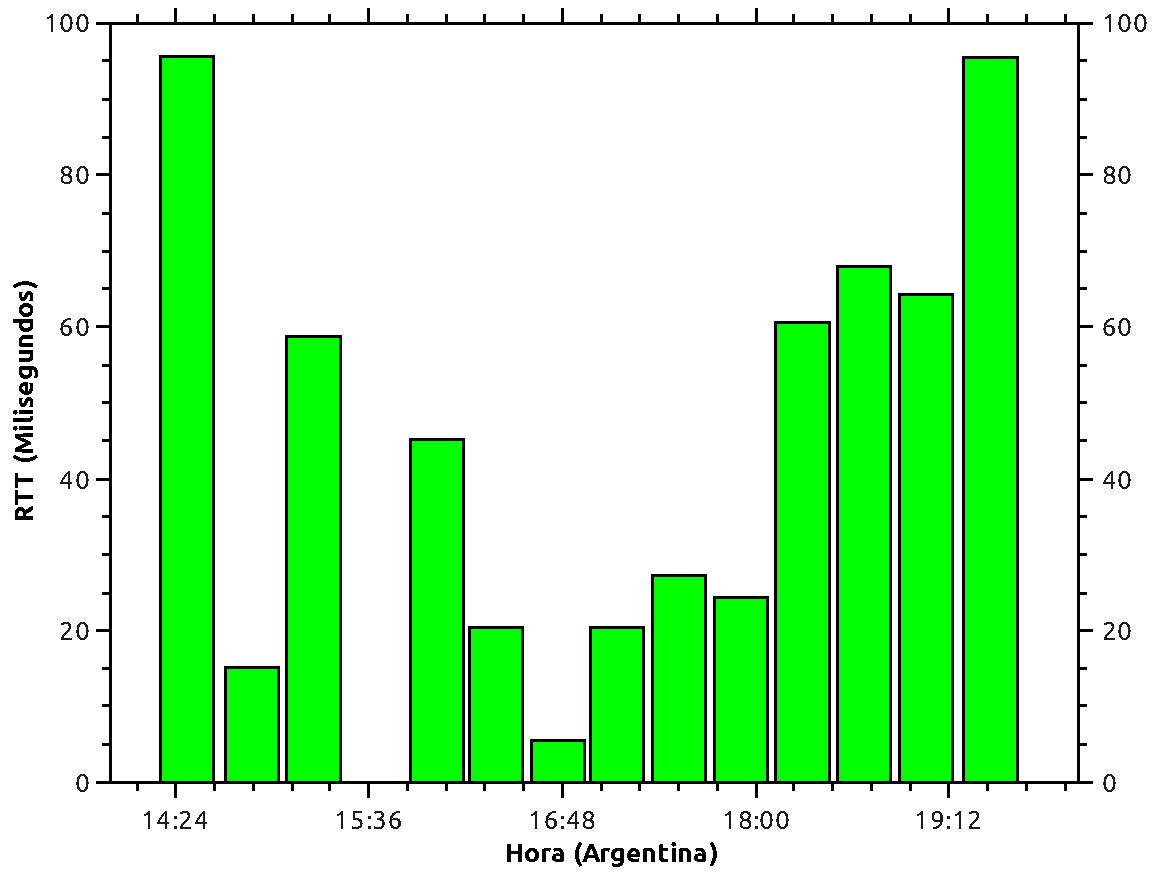
\includegraphics[width=0.9\textwidth]{graficos/rtts_dia_finlandia.pdf}
    \caption{RTTs medidos a lo largo del dia en el enlace EEUU-RU}
    \label{fig:rtts_fin}
\end{figure}

%EEUU : -3
%FINLANDIA: +4

En la figura \ref{fig:rtts_fin} se puede ver cómo los RTT varían constantemente durante todo el día, pricipalmente porque estos enlaces no sólo son utilizados por Estados Unidos, sino también por varios hosts ubicados en todo el continente americano. Debido a las difrencias horarias dentro del continente, es factible que mientras en algunos países el tráfico es muy intenso, en otros no sea esperable que se congestione la red. Calculamos la latencia de propagación del enlace (suponiendo que se extiende entre los puntos trazados y que se trata de un enlace de fibra óptica, de manera que la velocidad de propagación es de $2\cdot 10^{5}\frac{m}{s}$), para calcular un RTT mínimo como el doble de este tiempo (dado que los paquetes son pequeños, despreciamos el tiempo de transmisión). En este caso resultó de $75,44$ms que, en muchos casos, es mayor al RTT observado. Atribuimos esto a la inestabilidad de nuestro método de medición y la dificultad de determinar efectivamente la ubicación de los extremos del enlace.

De todas formas, pese a esto se pueden ver a grandes rasgos cómo a las 16hs de Argentina, el cual equivale a un rango de entre las 11hs y las 16hs de todo el continente americano, este enlace parece estar mucho menos congestionado que entre las 16 y las 20hs. 

%%% Aca hay q pulirlo.. esta medio chori.. le falta poder de sintesis :P, capas meter alguna tabla con zonas horarias.. y sacar alguna conclusion de trafico segun momento del dia..

*** ACLARAR RTTS NEGATIVOS


\begin{figure}[H]
  \centering
    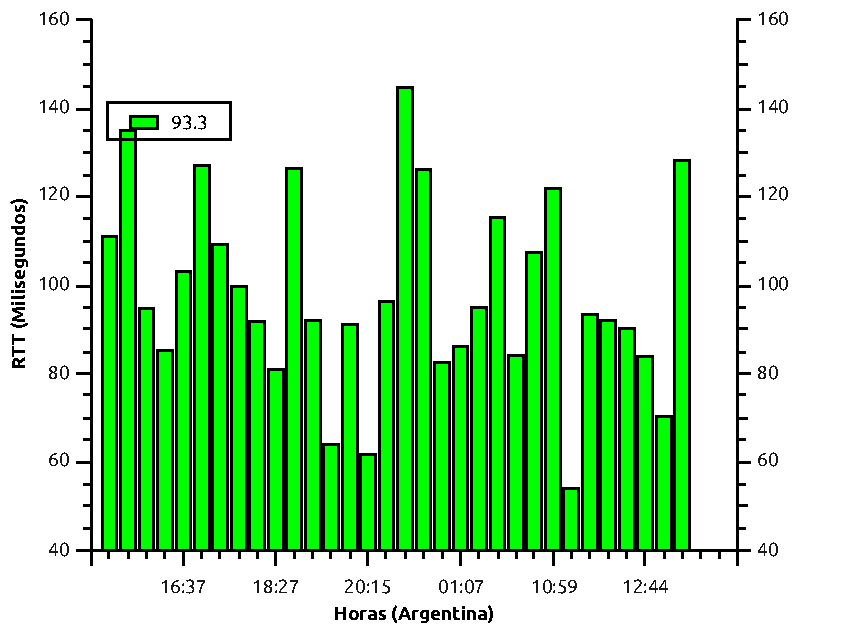
\includegraphics[width=0.9\textwidth]{graficos/rtts_dia_inglaterra.pdf}
    \caption{RTTs medidos a lo largo del dia en un enlace de EEUU - Alemania}
    \label{fig:rtts_ing}
\end{figure}

En el caso de la figura \ref{fig:rtts_ing} se puede ver que, si bien se observan picos en los horarios laborables, durante el resto del día no existe una tendencia o valor representativo. Este es un ejemplo de lo caótico e irregular que puede llegar a ser el tráfico en Internet. El mismo cálculo de RTT mínimo del caso anterior resulta aquí en $82,47$ms que parece ser un resultado más acertado. Observamos que todas las mediciones están por arriba, algunas de ellas considerablemente. Más allá de la inestabilidad manifestada anteriormente, aquí podemos ver que la mayoría de las mediciones resultan entre $80$ms y $100$ms, lo que evidencia que, para comunicaciones de realmente larga distancia, el factor geográfico sigue siendo el mayor limitante en cuando a la demora promedio (por sobre los tiempos de demora de funcionamiento del protocolo en sí, como por ejemplo, las colas de los routers y las decisiones de routeo).